\documentclass[12pt]{article}

%----------------------------------------------------------------------------------------
%	PACKAGES
%----------------------------------------------------------------------------------------

\usepackage{cite}
\usepackage{graphicx}
\usepackage{caption}
\usepackage{subcaption}
\usepackage{amssymb}
\usepackage{mathtools}
\usepackage{amsmath}
\usepackage{isomath}
\usepackage{hyperref}
\usepackage[hypcap]{caption}
\usepackage{listings}
\usepackage{color}

%----------------------------------------------------------------------------------------
%	PAGE & LINKS SETUP
%----------------------------------------------------------------------------------------

% Default margins are too wide all the way around. I reset them here
\setlength{\topmargin}{-.5in}
\setlength{\textheight}{9in}
\setlength{\oddsidemargin}{.125in}
\setlength{\textwidth}{6.25in}

% Graphics folder path
\graphicspath{ {./images/} }

% Hyperlinks and URL setup
\hypersetup{
    bookmarks=true, % show bookmarks bar?
    unicode=false, % non-Latin characters in Acrobat’s bookmarks
    pdftoolbar=true, % show Acrobat’s toolbar?
    pdfmenubar=true, % show Acrobat’s menu?
    pdffitwindow=false, % window fit to page when opened
    pdfstartview={FitH}, % fits the width of the page to the window
    pdftitle={IDAPI Coursework 2}, % title
    pdfauthor={Hesam Ipakchi, Yijie Ge}, % author
    pdfsubject={IDAPI Coursework 2}, % subject of the document
    pdfcreator={Hesam Ipakchi}, % creator of the document
    pdfproducer={Hesam Ipakchi, Yijie Ge}, % producer of the document
    pdfkeywords={Hesam Ipakchi, Yijie Ge, IDAPI Coursework 2}, % list of keywords
    pdfnewwindow=true, % links in new window
    colorlinks=true, % false: boxed links; true: colored links
    linkcolor=red, % color of internal links (change box color with linkbordercolor)
    citecolor=blue, % color of links to bibliography
    filecolor=black, % color of file links
    urlcolor=black  % color of external links
}
\urlstyle{same}

% Subreferences Setup
\captionsetup{subrefformat=parens}

%----------------------------------------------------------------------------------------
%	DEFINITIONS OF NEW COMMANDS
%----------------------------------------------------------------------------------------


%----------------------------------------------------------------------------------------
%	BEGIN DOCUMENT
%----------------------------------------------------------------------------------------

\begin{document}

% Consider all references (including those not cited) for biliography
\nocite{*}

%----------------------------------------------------------------------------------------
%	TITLE PAGE
%----------------------------------------------------------------------------------------

\title{\textbf{Intelligent Data Analysis and Probabilistic Inference Coursework 2}}
\author{Hesam Ipakchi (00648378), Yijie Ge (00650073)\\Imperial College London}
\date{\today}
% make title page without page number in footer
\clearpage\maketitle
\thispagestyle{empty}

%----------------------------------------------------------------------------------------
%	RESULTS
%----------------------------------------------------------------------------------------

\newpage
\thispagestyle{plain}
\mbox{}

% start page numbers arabic style (1,2,3...)
\pagenumbering{arabic} 

\section {IDAPIResults02.txt File Contents}
\label{sec:resultsFileContents}

\lstinputlisting{IDAPIResults02.txt}

%----------------------------------------------------------------------------------------
%	MAXIMALLY WEIGHTED SPANNING TREE
%----------------------------------------------------------------------------------------

\newpage
\thispagestyle{plain}
\mbox{}

\section {Maximally Weighted Spanning Tree}
\label{sec:maximallyWeightedSpanningTree}

\begin{figure}
	\centering
	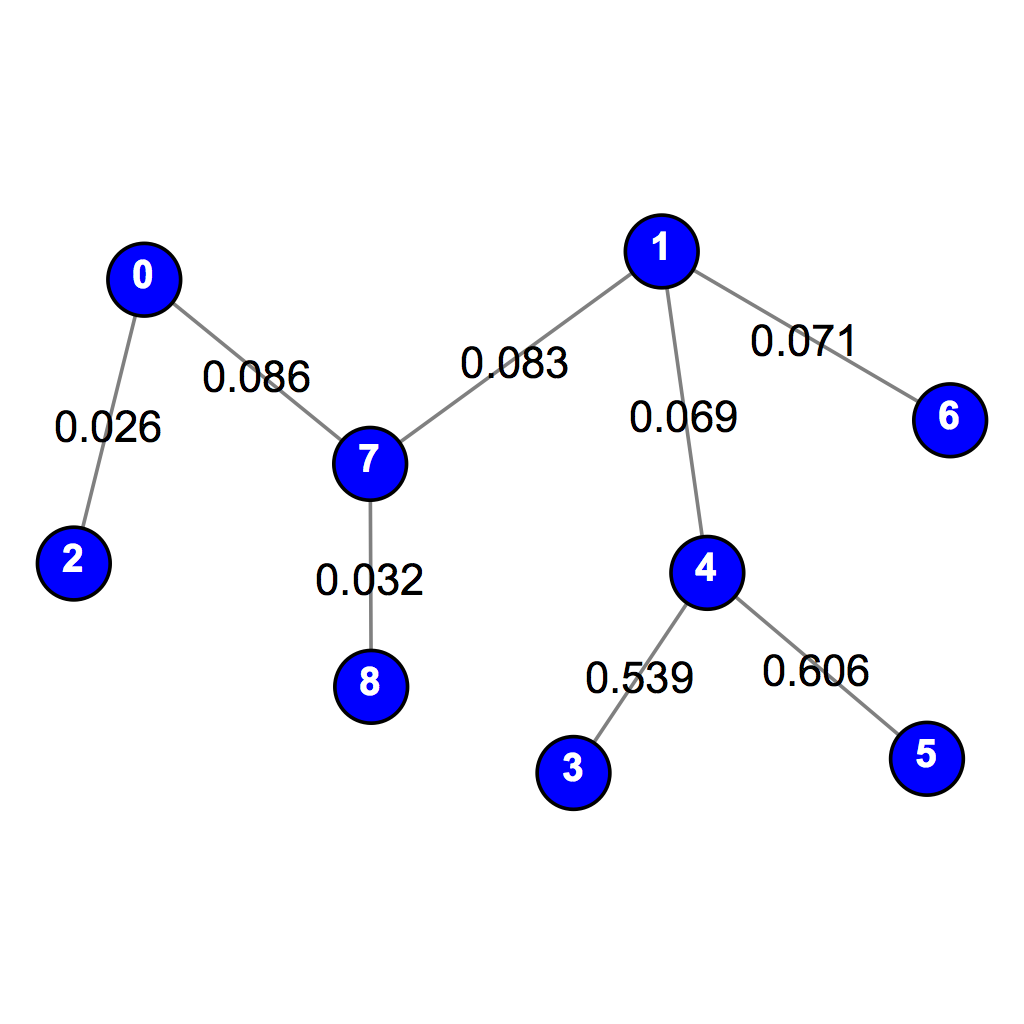
\includegraphics[width=0.8\linewidth]{spanningTree.png}
	\caption[Maximally Weighted Spanning Tree obtained from HepatitisC data set]{\label{fig:maximallyWeightedSpanningTree} Maximally Weighted Spanning Tree obtained from HepatitisC data set.}
\end{figure}

See Figure \ref{fig:maximallyWeightedSpanningTree} for the maximally weighted spanning tree we obtained. Nodes are coloured blue and indexed from 0 to 8; whilst edges are grey with the dependency between the two nodes connected by the edge written on it.

\end{document}